\chapter{System Design and Architecture}
\label{chapter:architecture}

Design and architecture constitute critical determinants of the \ac{splash} system's functionality, efficiency, and scalability. This section details the foundational components of the \ac{splash} proof-of-concept, demonstrating the integration of elements to create a cohesive solution for a beach preventive safety management. \\
Key diagrams illustrate the system’s architecture and operational framework. Each diagram provides unique insight into specific aspects of the system, clarifying its structure and functional relationships. \\
Analysis of these diagrams advances understanding of the \ac{splash} system’s design principles and operational capabilities, establishing a basis for further investigation into implementation and potential contributions.

\newpage
\section{Context Diagram}
\label{section:context_diag}

The context diagram in Figure \ref{fig:context_diag} defines the system’s boundaries and interactions with external entities, including users, environmental sensors, emergency services, and third-party data providers. It clarifies input/output flows, such as hazard alerts, sensor data streams, and user requests, while omitting internal implementation details. This diagram establishes the scope of the \ac{splash} system within the broader beach safety ecosystem.

The context diagram in Figure \ref{fig:context_diag} describes the \ac{splash} system’s boundaries and its interactions with key external stakeholders such as Supervisor Lifeguards, Regular Lifeguards, Beachgoers, and Beach Business Owners (concessionaires). The diagram illustrates the bidirectional flow of generic information, such as new updates, authorized beach information, and business metrics, between the system and each external entity. By mapping these exchanges, the diagram clarifies the roles and data dependencies of all parties involved, while abstracting away internal system details. This representation defines the operational scope of the \ac{splash} system within the management environment of a beach.

\begin{figure}[H]
      \centering
      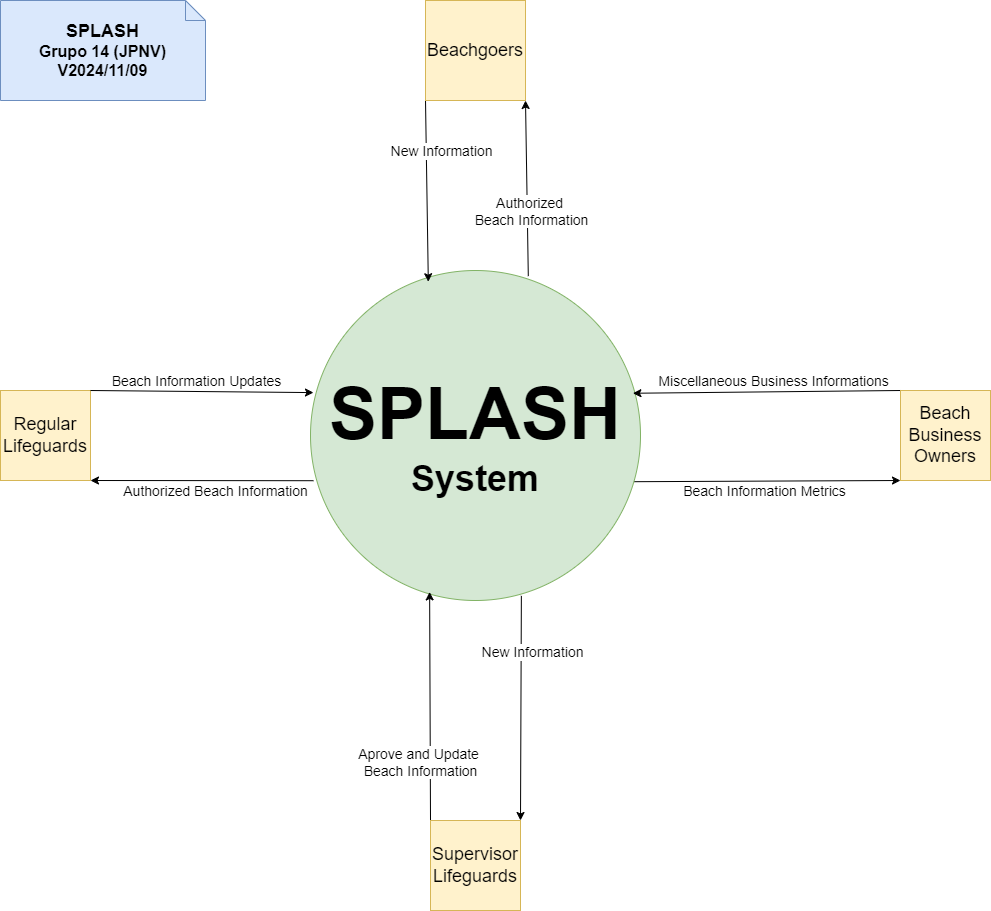
\includegraphics[width=15cm]{figs/context_diagram.png}
      \caption{ \textbf{\ac{splash} System Context Diagram:} For a detailed, full-resolution version, visit: \url{https://github.com/SPLASHub/SplashDocumentation/}}
      \label{fig:context_diag}
\end{figure}

\newpage
\section{High-Level Architecture Diagram}
\label{section:high_level_diag}

Figure \ref{fig:high_level_diag} illustrates the system’s core architectural layers: the Presentation Layer and each interface, the Program Logic Layer and the Data Layer with persistent data storage. The diagram depicts flow of requests and responses between users, interface components, backend modules, and the database. This design allows for easy future updates and growth (scalability), allowing new features and components to be integrated smoothly as the system evolves.

\begin{figure}[H]
      \centering
      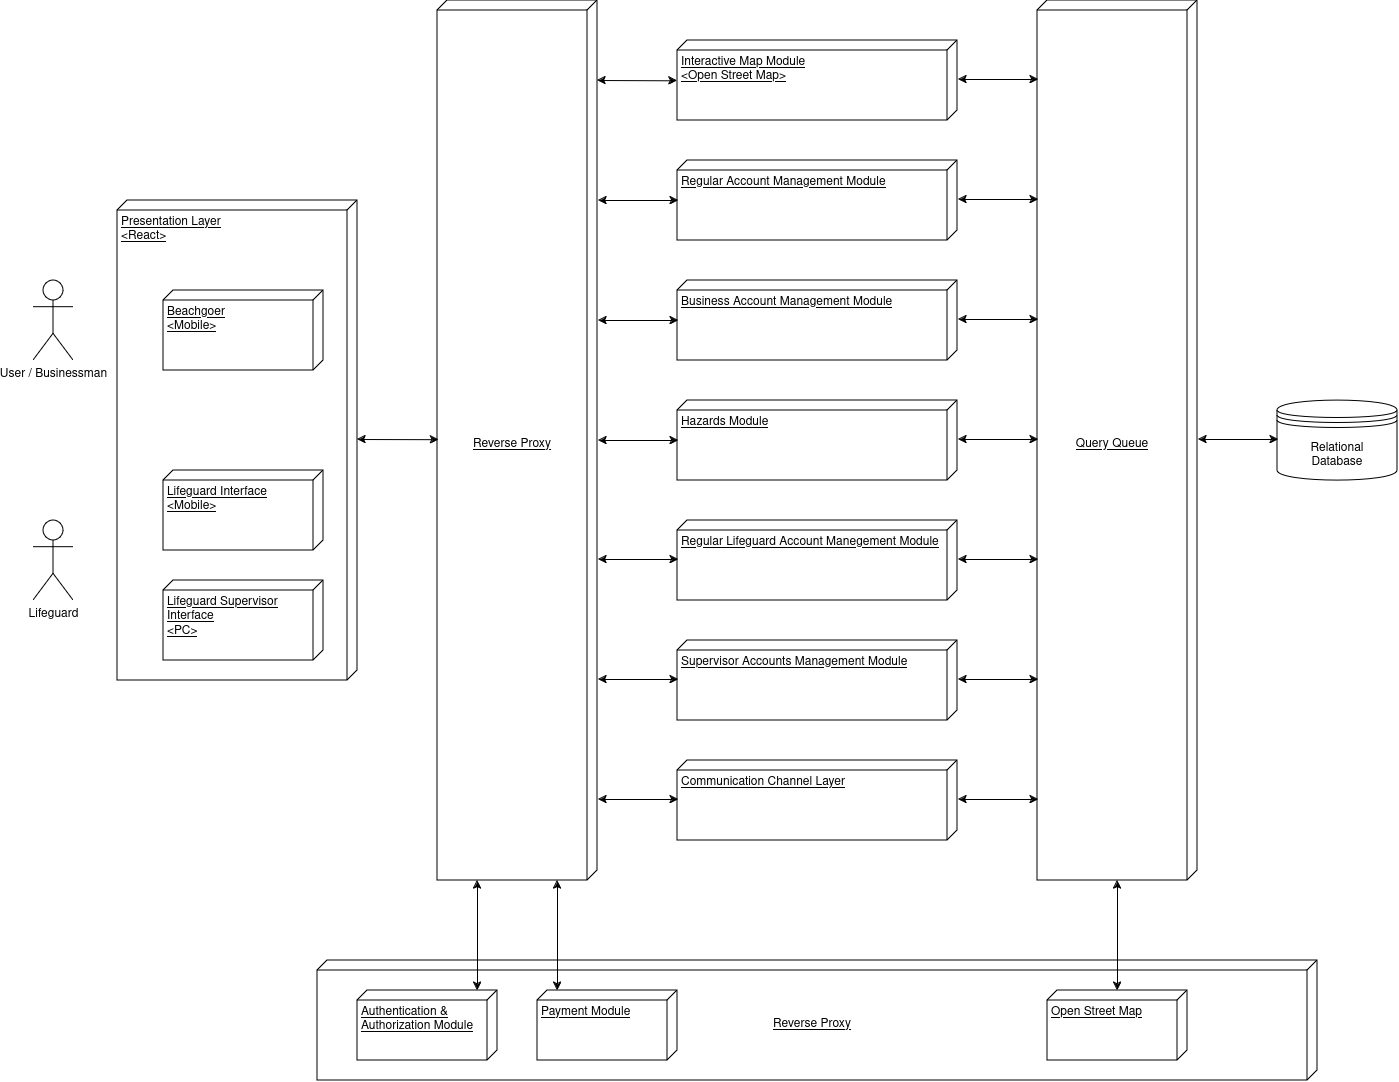
\includegraphics[width=16cm]{figs/diag_high_level.png}
       \caption{ \textbf{\ac{splash} High-Level Architecture Diagram:} For a detailed, full-resolution version, visit: 
       \url{https://github.com/SPLASHub/SplashDocumentation/}}
       \label{fig:high_level_diag}
\end{figure}

\newpage
\section{Use-Case Diagram}

The use-case diagram (Figure \ref{fig:use_case_diagram}) illustrates the main actors and their interactions with the \ac{splash} system. Regular users, lifeguards, supervisors and beach business owners each access different features, such as reporting hazards, managing teams, viewing beach information, and inputting data. External services handle authentication and payments. The diagram highlights how each actor accesses relevant system functions, with clear boundaries and relationships between use cases.

\begin{figure}[H]
      \centering
      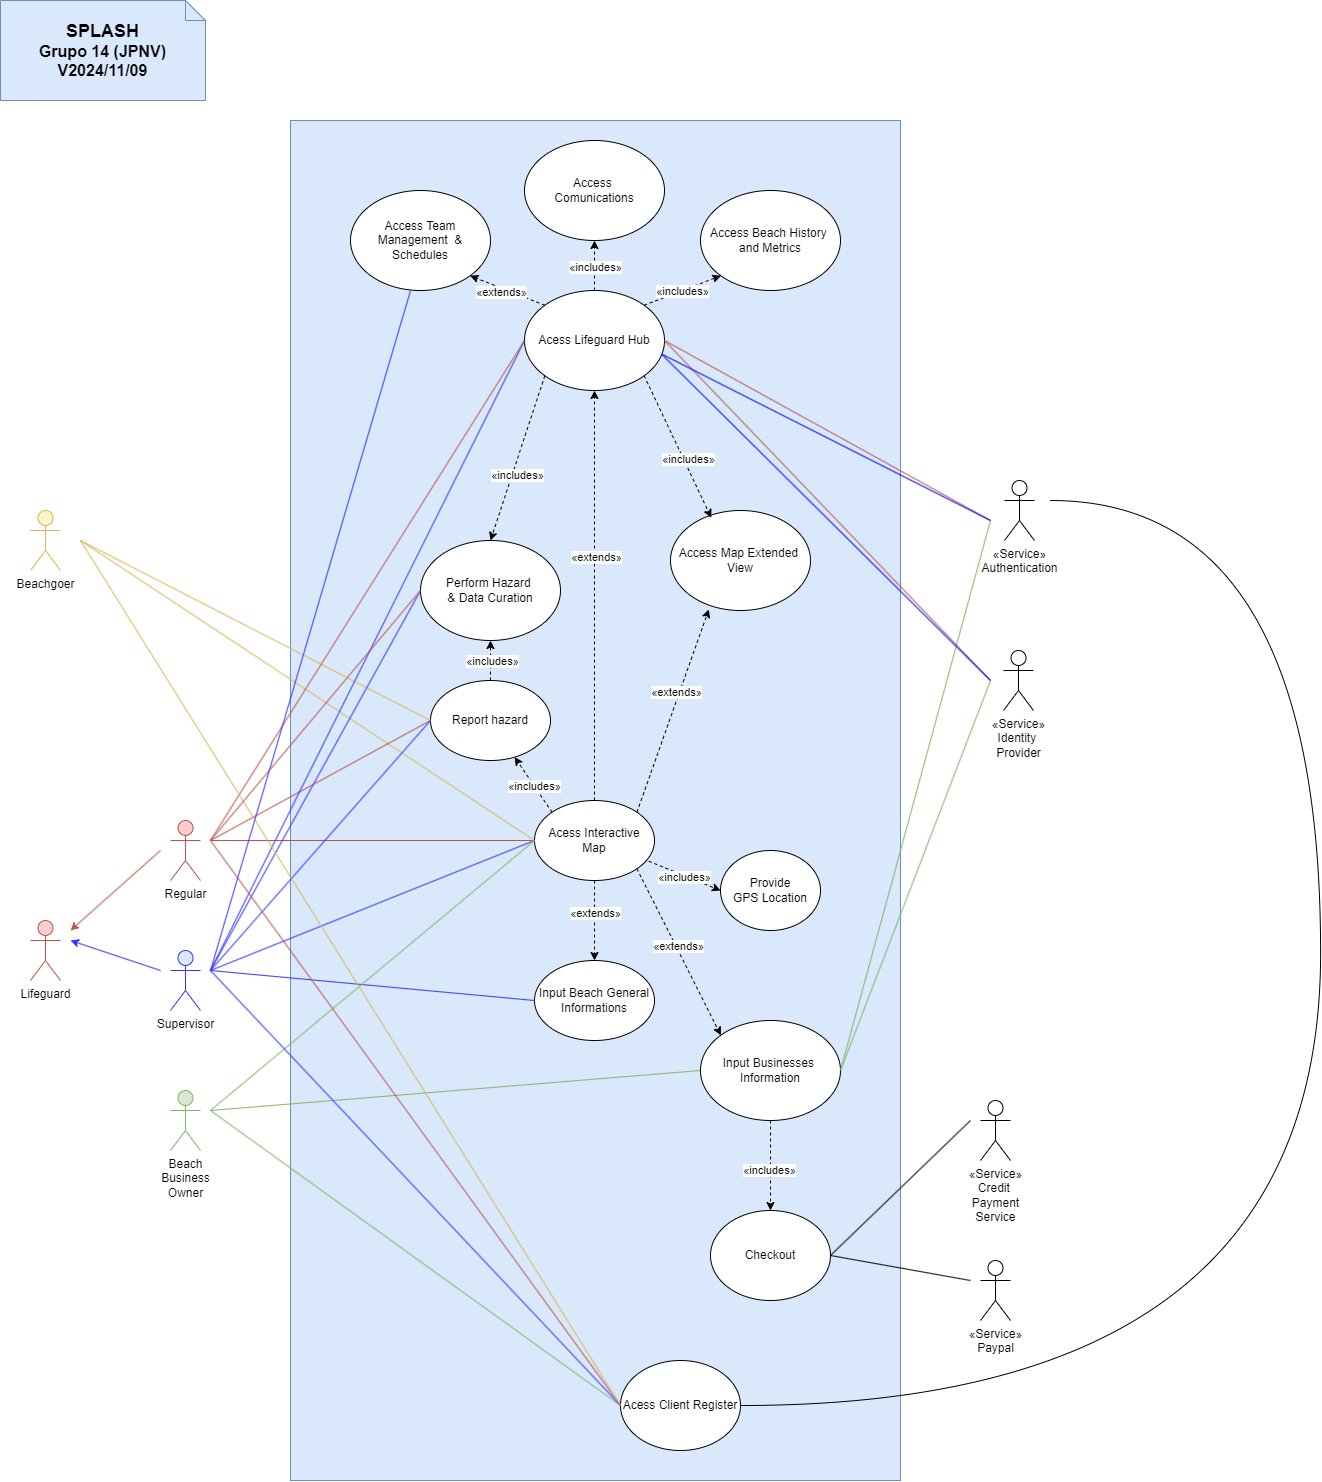
\includegraphics[width=16cm]{figs/use_case_diagram.png}
      \caption{ \textbf{\ac{splash}: System Use-Case Diagram:} For a detailed, full-resolution version, visit: 
      \url{https://github.com/SPLASHub/SplashDocumentation/}}
      \label{fig:use_case_diagram}
\end{figure}

\newpage
\section{Components Diagram}

The system components diagram (Figure \ref{fig:componets}) shows the main architectural elements of the \ac{splash} system and their interactions. Wearable tracking devices with GPS and RFID modules communicate with the backend server through an API. The backend server manages data storage and retrieval via a connected database. Users interact with the system through web app interfaces, which are tailored for lifeguards, beachgoers and businesses, ensuring each role accesses the appropriate features.

\begin{figure}[H]
      \centering
      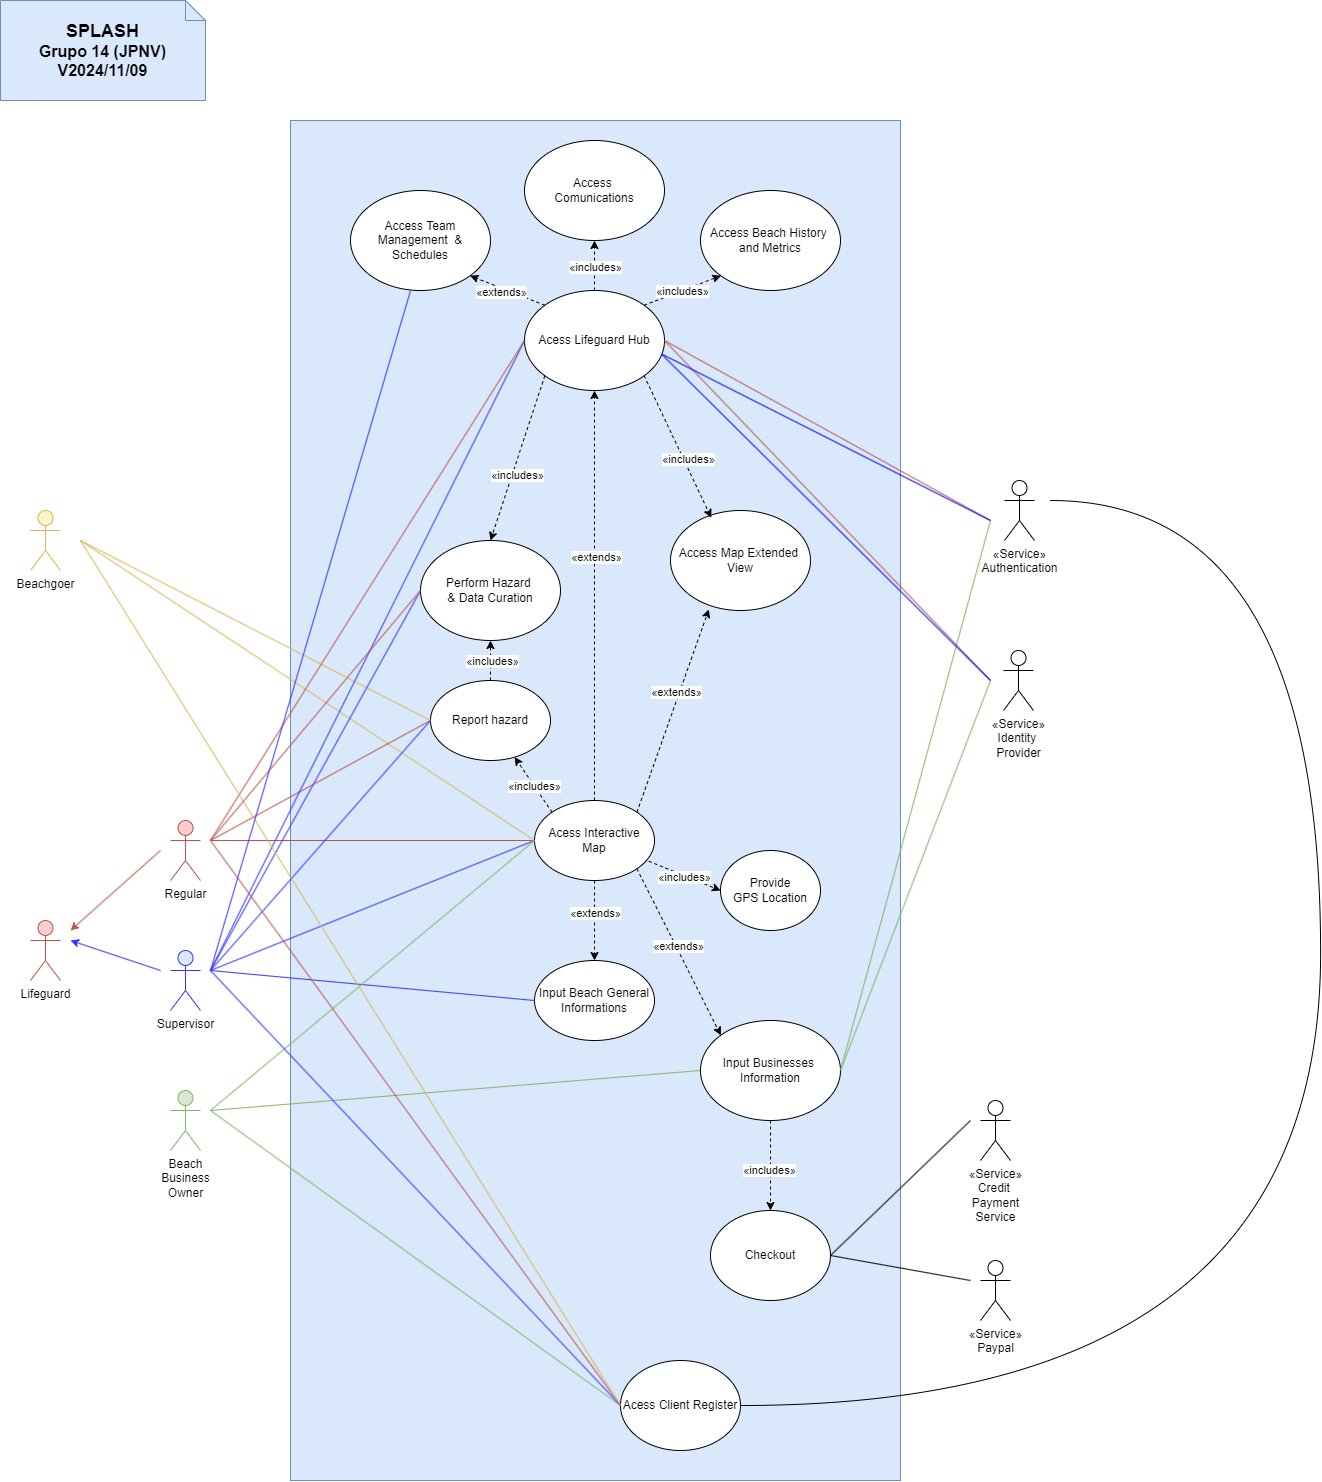
\includegraphics[width=16cm]{figs/use_case_diagram.png}
      \caption{ \textbf{\ac{splash}: System Components Diagram:} For a detailed, full-resolution version, visit: 
      \url{https://github.com/SPLASHub/SplashDocumentation/}}
      \label{fig:componets}
\end{figure}

\newpage
\section{Data Flow Diagram}

The data flow diagram (Figure~\ref{fig:data_flow}) provides an overview of how information moves through the \ac{splash} system. It details the interactions between key external entities (users, lifeguards, etc...) and the system’s main processes, including hazard reporting, team management, beach information access, and payment handling. The diagram illustrates how data is collected, processed, stored, and shared across different modules.

\begin{figure}[H]
      \centering
      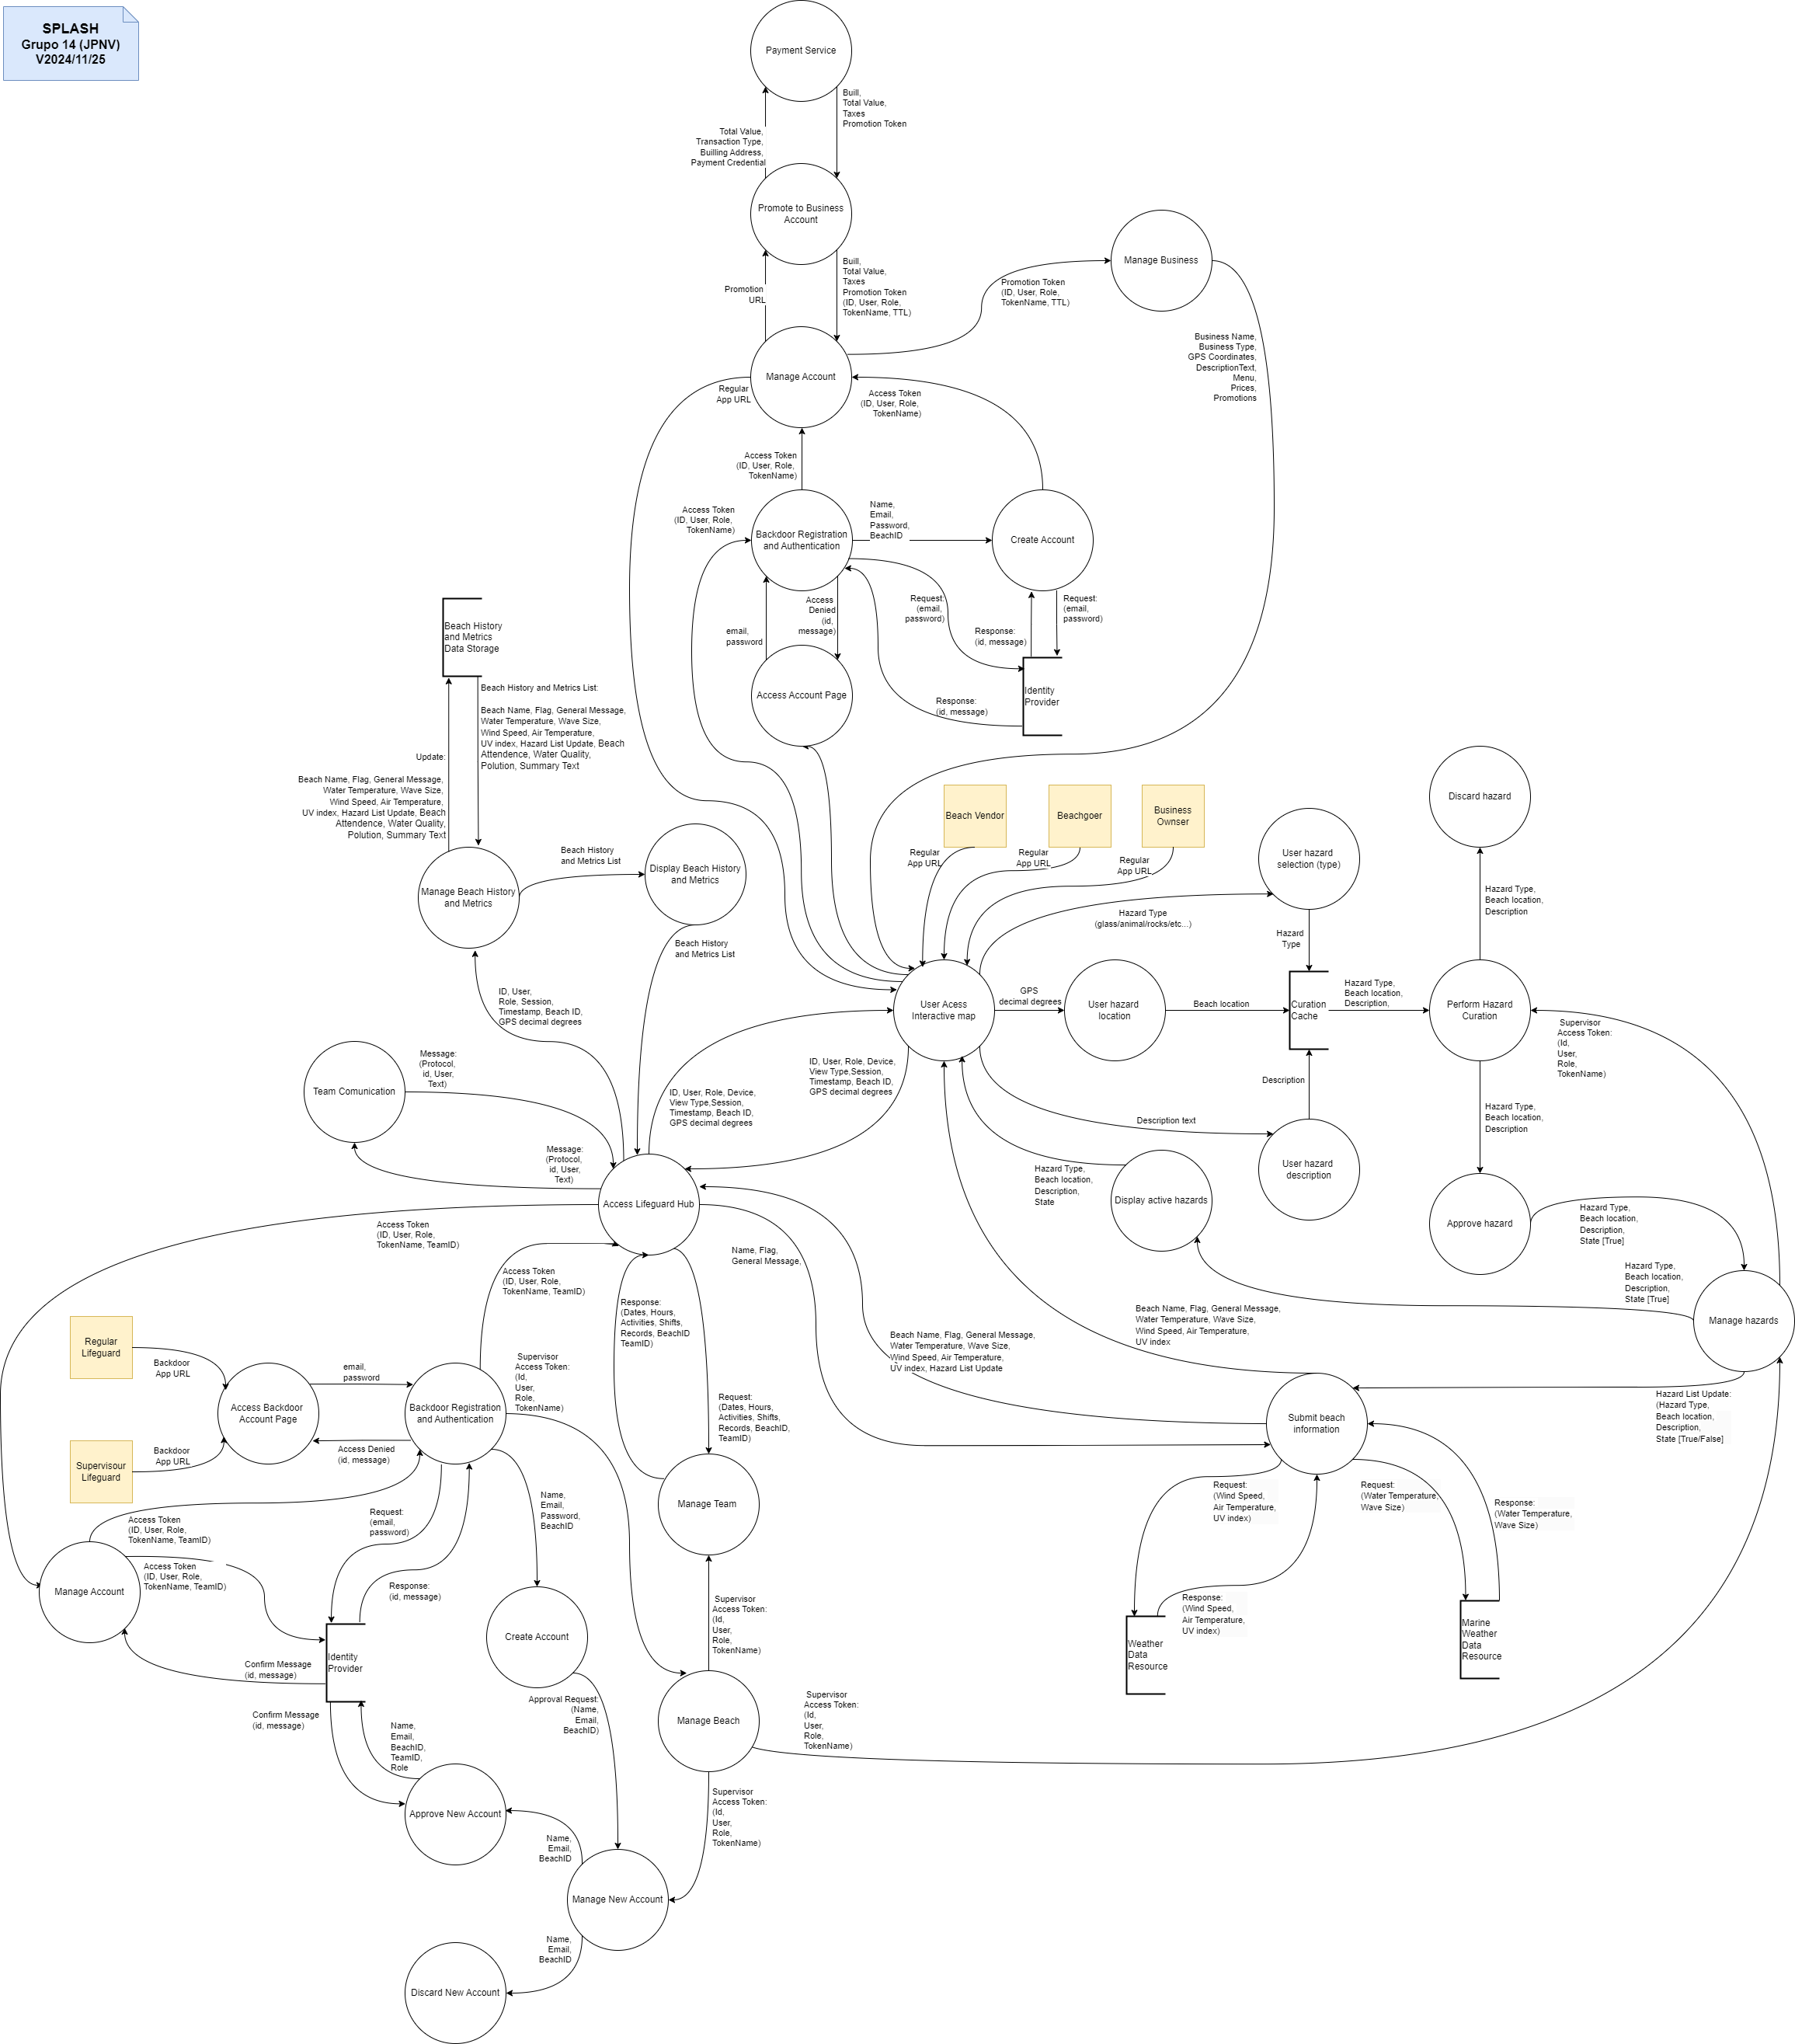
\includegraphics[width=16cm]{figs/data_flow.png}
      \caption{ \textbf{ \ac{splash}: System Data Flow Diagram:}  For a detailed, full-resolution version, visit: 
      \url{https://github.com/SPLASHub/SplashDocumentation/}}
      \label{fig:data_flow}
\end{figure}

\newpage
\section{Deployment Diagram}

Figure \ref{fig:deployment} illustrates the deployment architecture of the \ac{splash} system, showcasing the interaction between different hardware and software components in a real-world environment.

The system consists of three primary components:
\begin{itemize}
    \item \textbf{Wearable Device}: Equipped with GPS/RFID tracking capabilities, this device communicates wirelessly with the backend server to provide location and tracking data.
    
    \item \textbf{User Devices}: These include web-based interfaces. These devices communicate with the backend server using REST APIs or WebSocket protocols.
    
    \item \textbf{Backend Server}: Hosts multiple services, including an API Service for handling requests, a Notifications Engine for managing alerts, and a Device Management module. The backend server interacts with an SQL database to store and retrieve relevant data using standard protocols.
\end{itemize}


\begin{figure}[H]
      \centering
      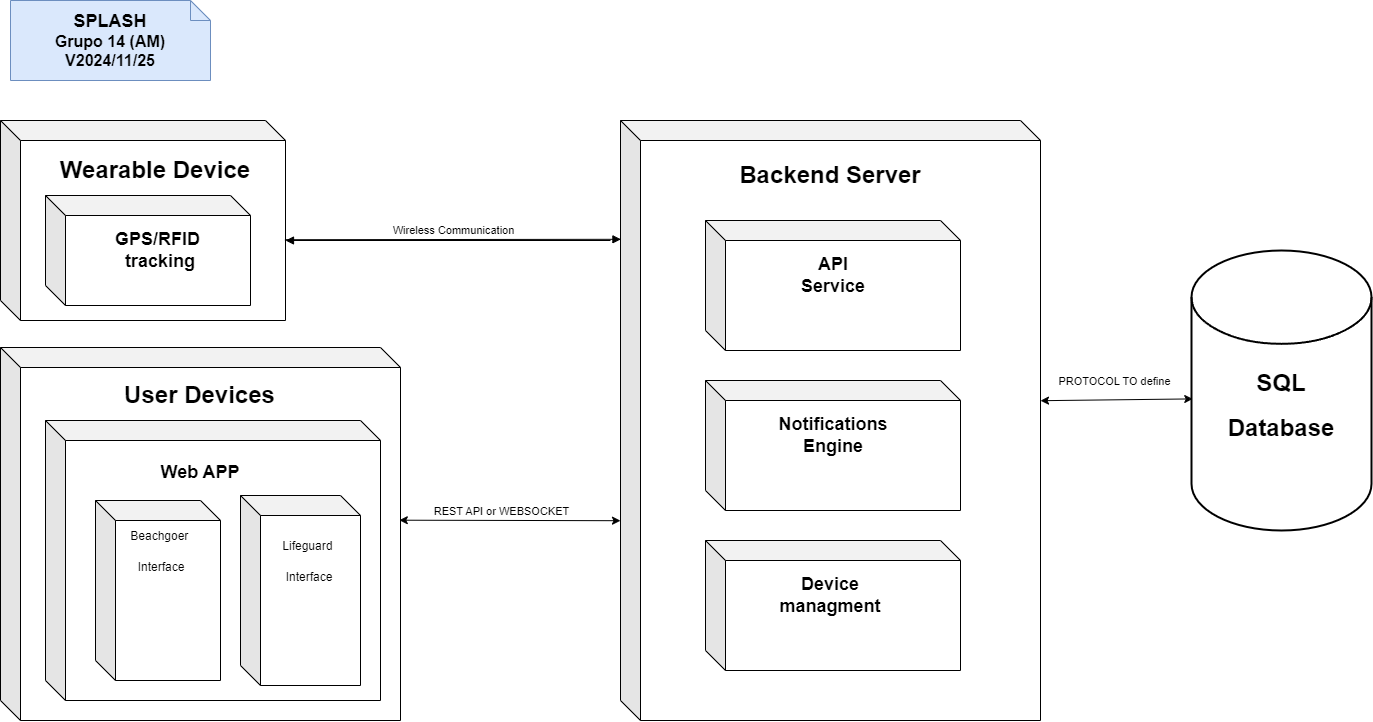
\includegraphics[width=16cm]{figs/deployment.png}
      \caption{ \textbf{ \ac{splash}: System Deployment Diagram: } For a more detailed view: \url{https://github.com/SPLASHub/SplashDocumentation/}}
      \label{fig:deployment}
\end{figure}

\newpage
\section{General Architecture Diagram}

Figure \ref{fig:general_architecture} provides a comprehensive overview of the \ac{splash} system architecture. It integrates all functional modules and services into a single schematic.

Key components include:
\begin{itemize}
    \item \textbf{Authentication \& Authorization Module}: Manages user access roles and account provisioning, ensuring secure access to the system.
    
    \item \textbf{Tracking Services}: Utilizes RFID and GPS to provide real-time location data for users and devices.
    
    \item \textbf{Interactive Map Module}: Integrates OpenStreetMap for visualization, allowing users to interact with geographic data.

    \item \textbf{Payment Module}: Supports transaction processing and account upgrades.

    \item \textbf{Presentation Views Layer}: Offers tailored interfaces for different user roles—Lifeguards, Supervisors, and Regular Users—with optimized map views and tool access.
    
    \item \textbf{Reverse Proxy}: Acts as the central routing mechanism that coordinates requests and responses between the view layer and backend services.

    \item \textbf{Query Queue \& Scalable Database}: Ensures efficient processing and persistent storage of requests and data through a queued system architecture.
\end{itemize}

\begin{figure}[H]
      \centering
      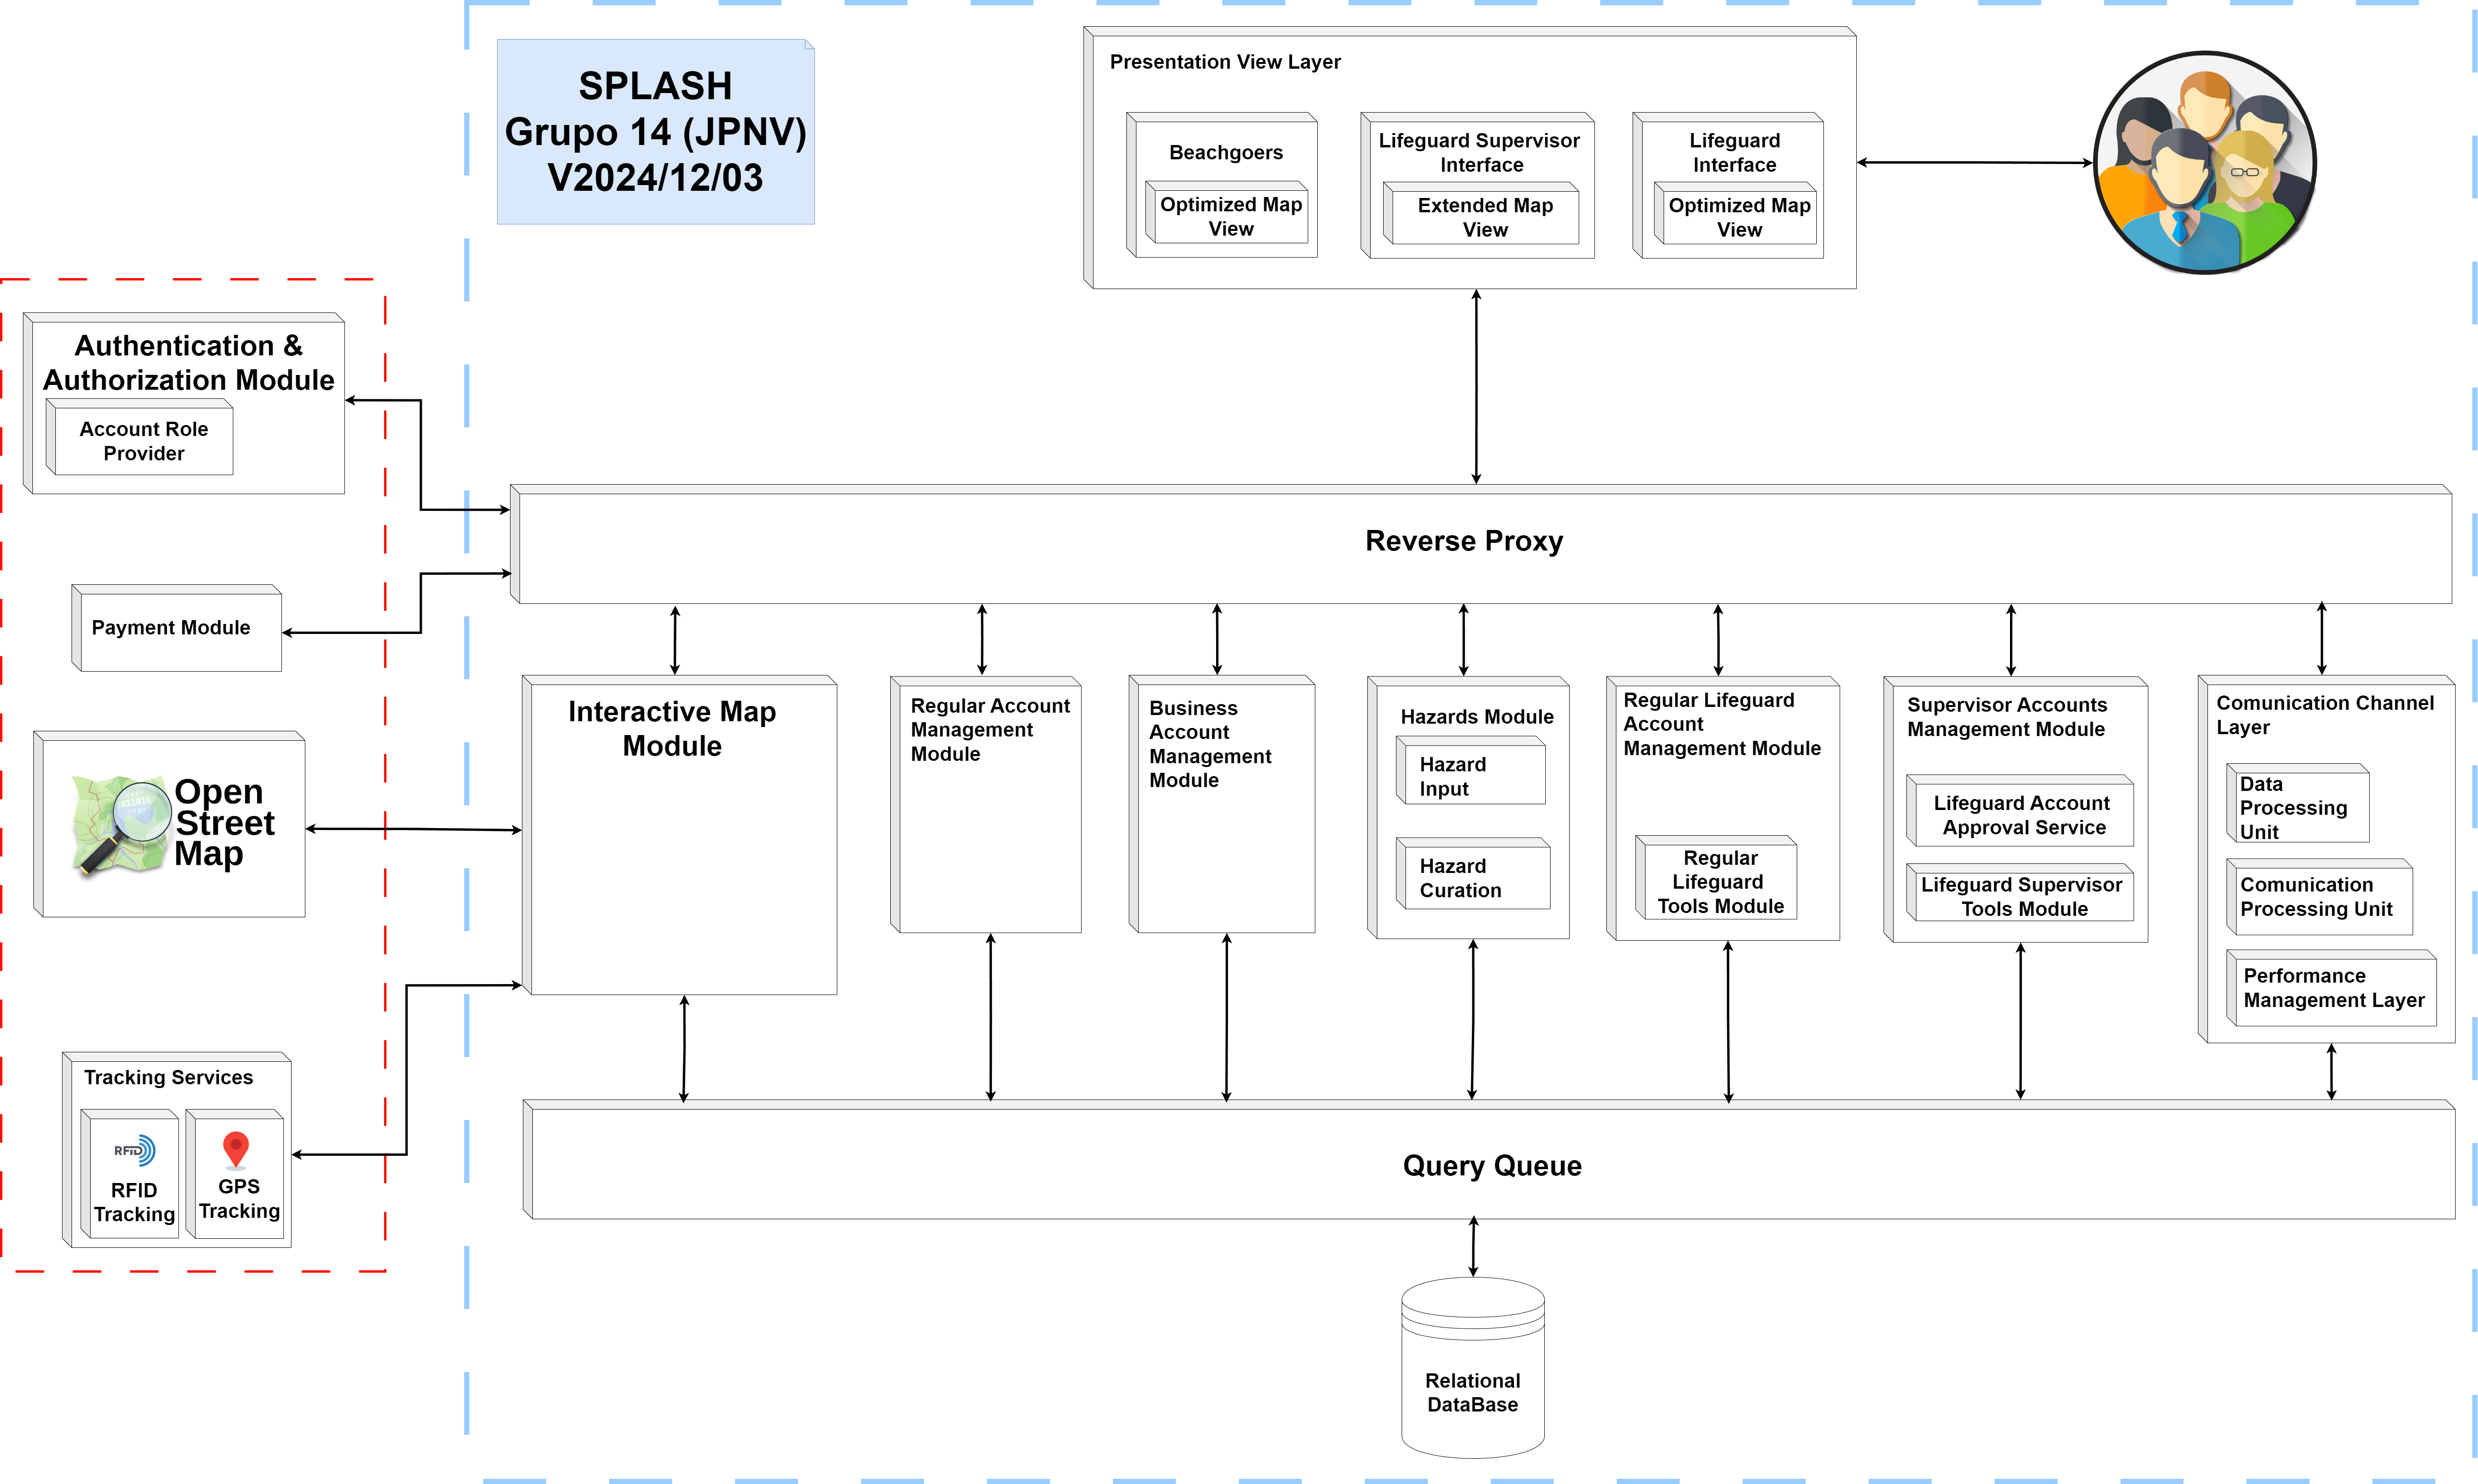
\includegraphics[width=16cm]{figs/general_architecture.png}
      \caption{ \textbf{ \ac{splash}: System General Architecture Diagram:} For a more detailed view: \url{https://github.com/SPLASHub/SplashDocumentation/}}
      \label{fig:general_architecture}
\end{figure}

\newpage
\section{Selected Technologies and Implementation}
\label{section:candidate_tech}

Following the development of the previous architectural diagrams and team discussions, a set of modern technologies was selected to implement the \ac{splash} system. The system architecture was designed as a web-based solution, integrating both hardware and software components for effective user interaction. \\
The \textbf{frontend} of the application was developed using \textbf{React}, chosen for its flexibility, reusable component structure, and ability to build dynamic and responsive user interfaces. \\
For the \textbf{backend}, \textbf{Visual Studio 2022} was employed to develop a RESTful API using \textbf{C\# and .NET}, which served as the bridge between the frontend, database, and wearable devices. This environment was selected for its robustness, development efficiency, and strong integration with cloud services. \\
A \textbf{relational database} was implemented using \textbf{PostgreSQL}, selected for its reliability, scalability, and ability to efficiently manage structured data and complex relationships between entities. \\

The \textbf{wearable devices}, developed as wristband prototypes specifically for children, integrate multiple technologies to ensure secure and reliable tracking. The core purpose of these devices is to provide real-time \textbf{geolocation data} exclusively to the legal guardians of the child, ensuring both safety and privacy. 
Each wristband prototype is built around the \textbf{ESP32-S3-WROOM-1} microcontroller, programmed using \textbf{PlatformIO} with the \textbf{ESP-IDF} framework. This microcontroller offers a powerful and energy-efficient solution for embedded IoT systems. For location tracking, the wristbands are equipped with a \textbf{NEO-6M GPS sensor}, enabling accurate and continuous geolocation updates. Communication with external devices is handled via the \textbf{Web Bluetooth API}, which allows for direct browser-based interaction without the need for native applications.

Finally, the entire system was deployed and hosted on the \textbf{Microsoft Azure} cloud platform. Azure was chosen for its scalability, reliability, and seamless support for .NET applications, ensuring that the system remains accessible and operational under varying loads. \\

This technology stack ensures that the \ac{splash} solution is robust, scalable, and user-centric, addressing the project’s core objectives while leveraging modern development practices to enhance safety, usability, and performance.

\begin{figure}[H]
    \centering
    \begin{subfigure}{0.48\textwidth}
        \centering
        
\includegraphics[width=\linewidth]{figs/Selected_Technologies.png}
        \caption{Selected Technologies for development}
        \label{fig:Selected_Technologies}
    \end{subfigure}
    \hfill
    \begin{subfigure}{0.48\textwidth}
        \centering
        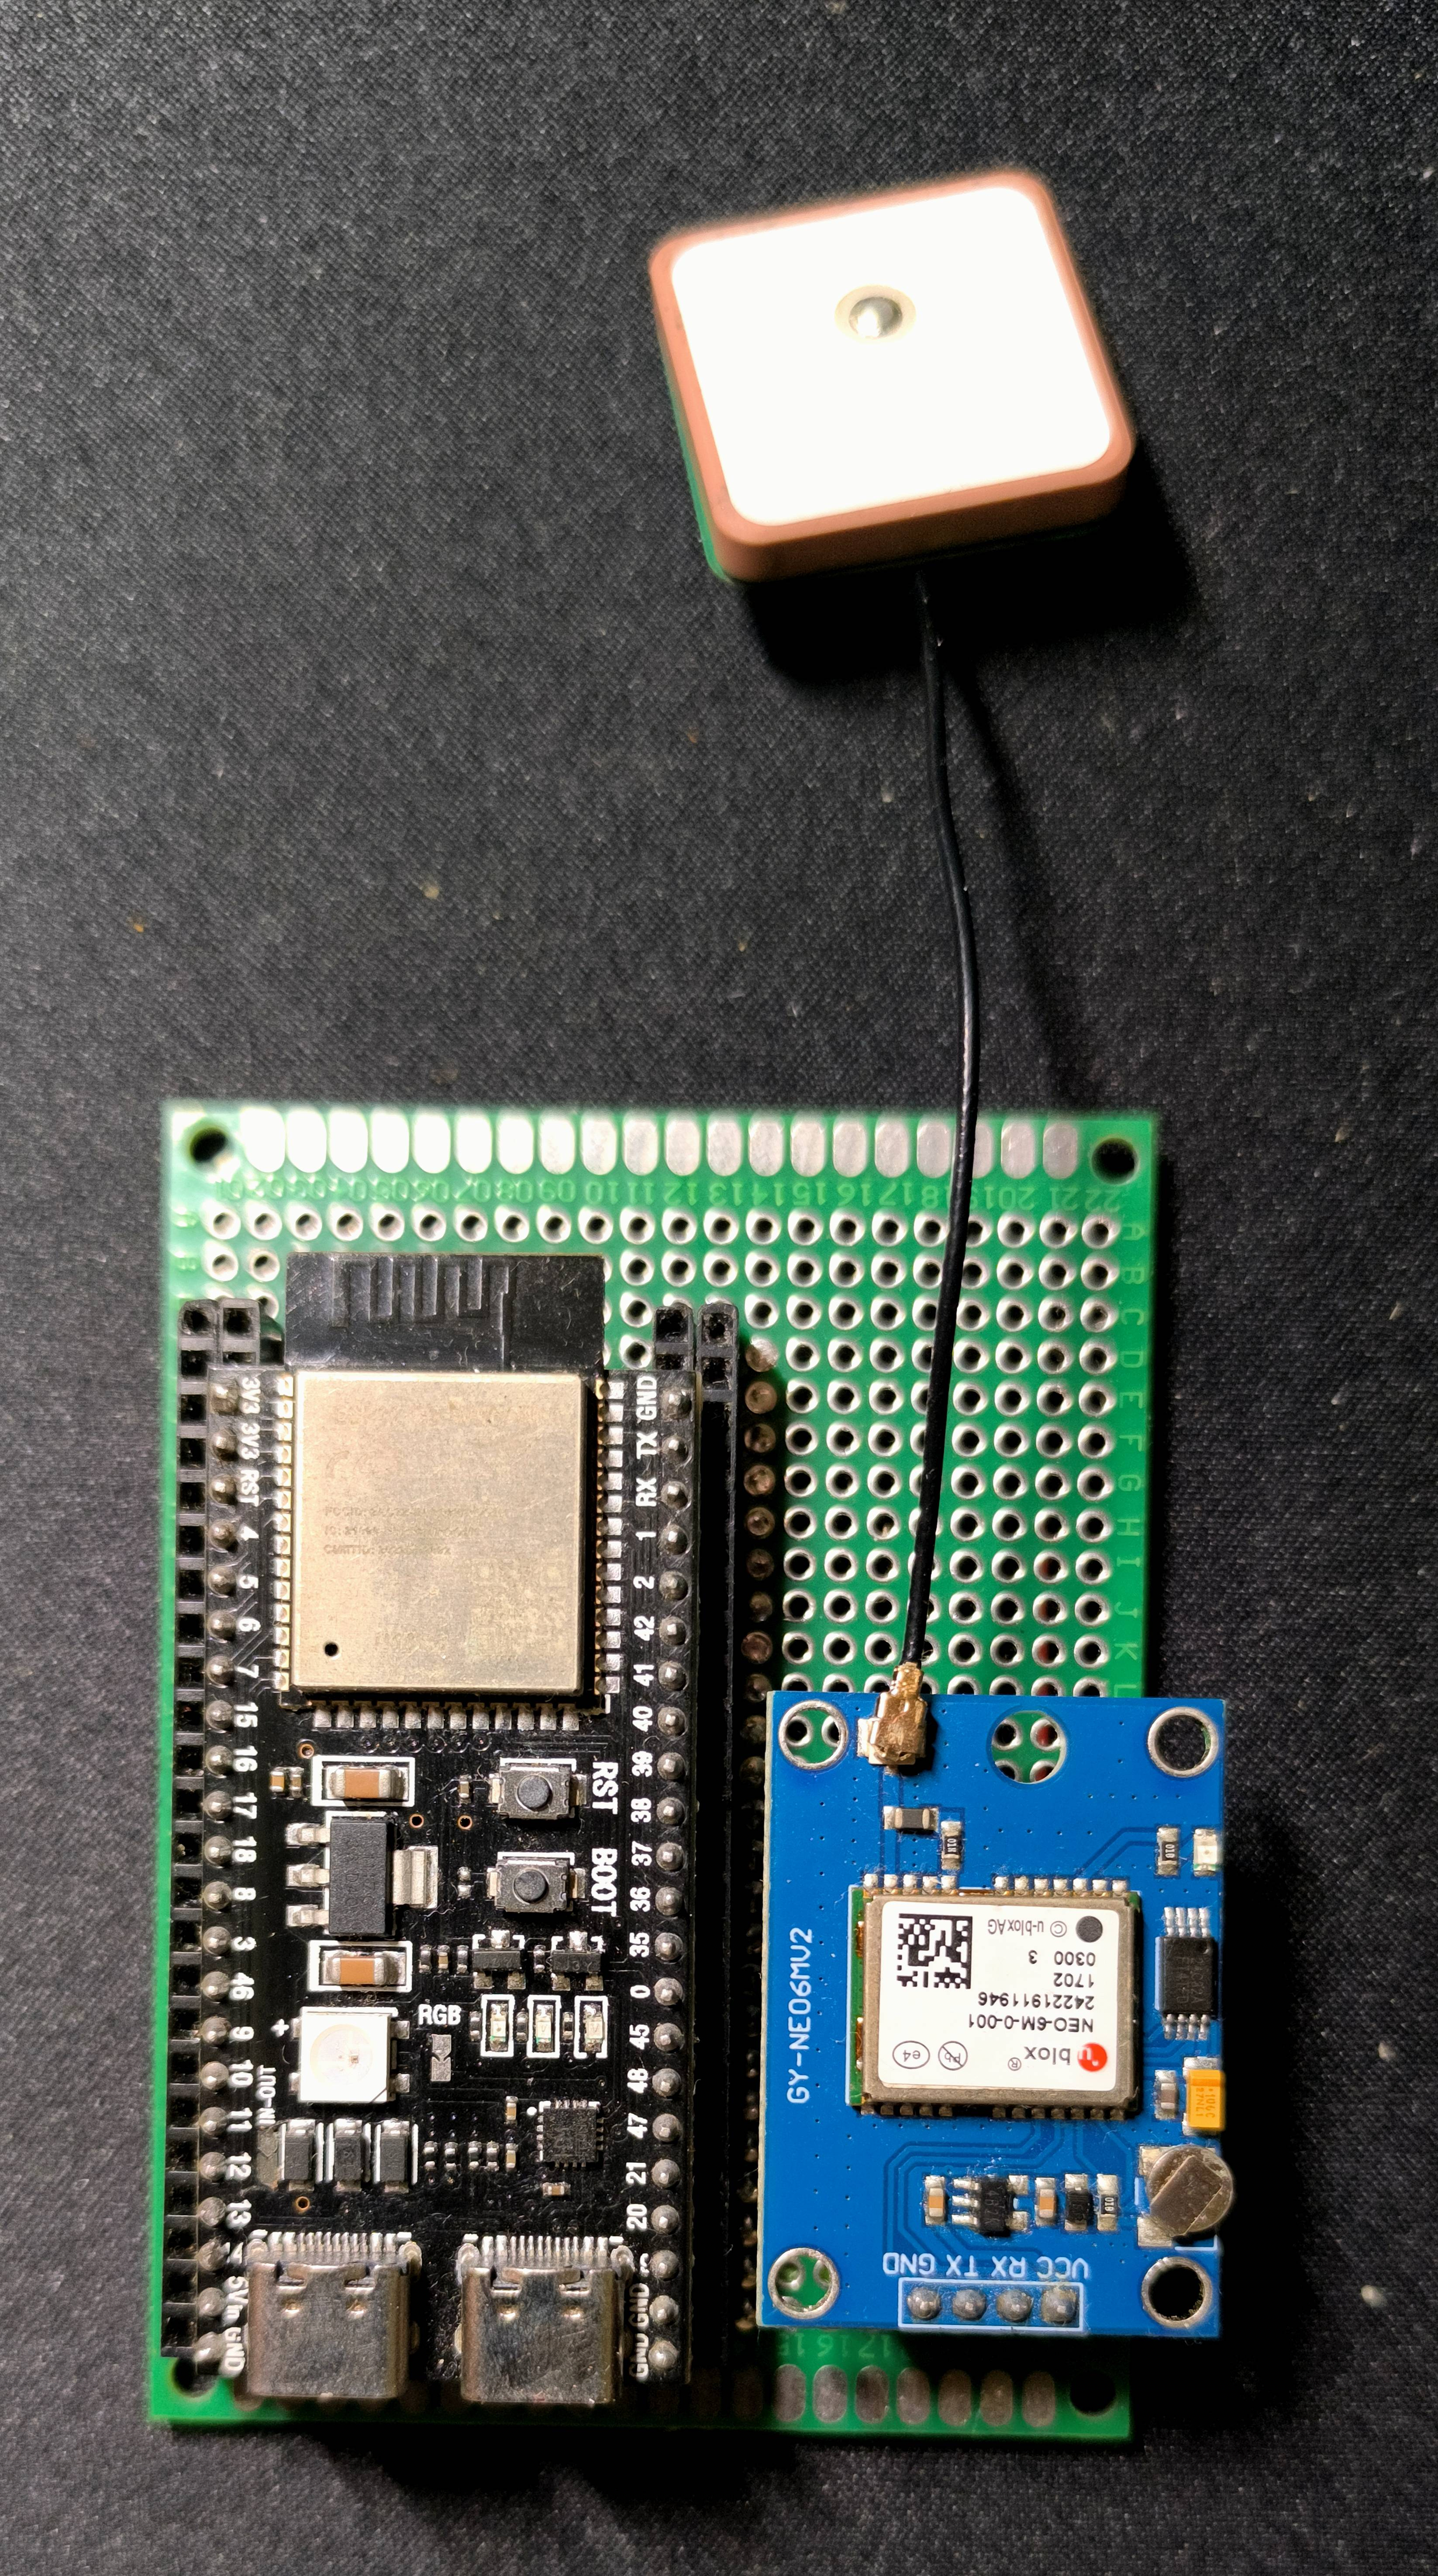
\includegraphics[width=0.4\linewidth,keepaspectratio]{figs/prototipo-pulseira.jpg}
        \caption{GPS wristband prototype}
        \label{fig:wristband_prototype}
    \end{subfigure}
    \caption{Overview of selected technologies and the prototype for the GPS wristband }
    \label{fig:technologies_and_prototype}
\end{figure}



\section{Database Design}
\label{section:dbdesign}

The \ac{splash} project employs a relational database management system (\ac{dbms}) as its core data infrastructure. This ensures structured, efficient, and scalable data storage, retrieval, and management to support the platform’s functionalities. The database is designed to maintain data integrity while allowing extensibility to support future enhancements and additional data sources such as smart devices. \\
The schema mirrors real-world entities involved in lifeguard operations, beach environments, and hazard management. Each table is uniquely identified using primary keys, while relationships between entities—such as users, lifeguards, beaches, and hazards are modeled using foreign keys, as illustrated in the Entity Relationship Diagram (Figure \ref{fig:DER}). This normalization focused design reduces redundancy, mitigates data anomalies, and allows easy data maintenance.

\subsection{Entity Relationship Diagram}
\label{subsection:DER}

\begin{figure}[H]
    \centering
    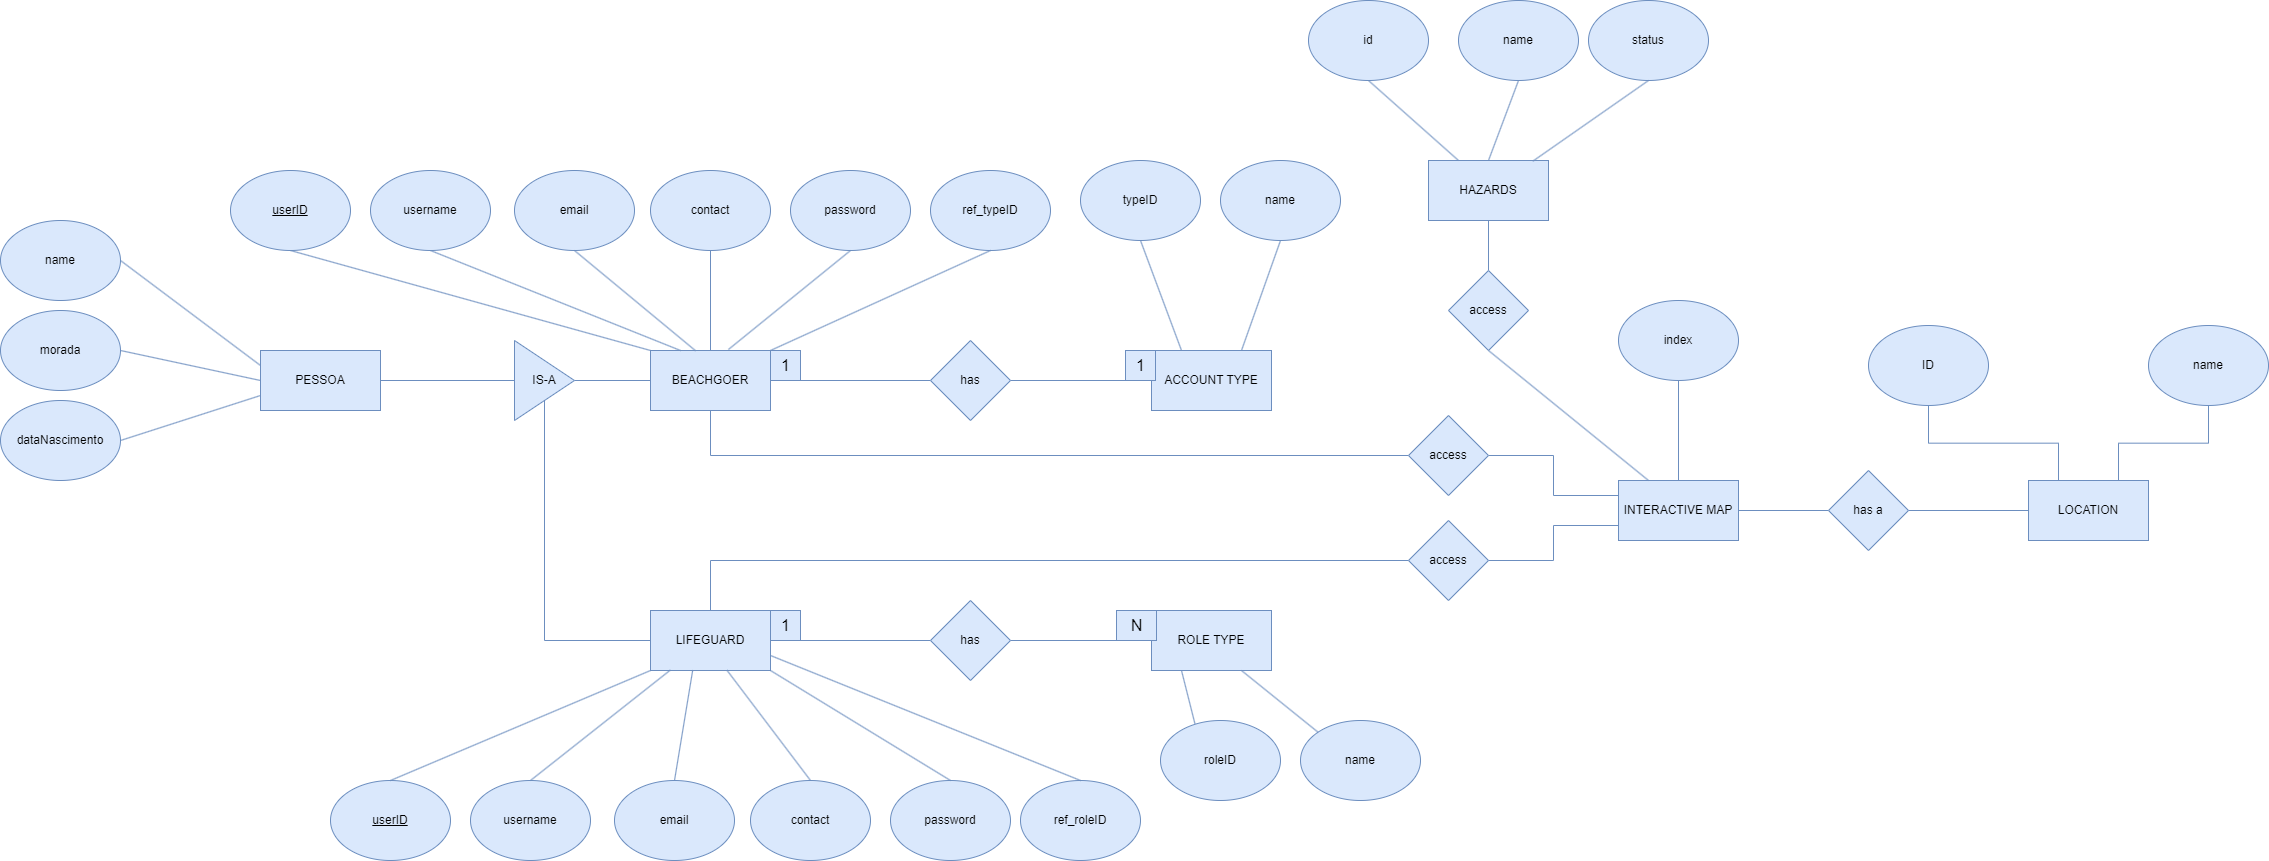
\includegraphics[width=16cm]{figs/DER.png}
    \caption{ \textbf{\ac{splash}: Entity Relationship Diagram:} The diagram presents the conceptual overview of the main entities and their relationships, laying the foundation for the database structure. For a more detailed view: 
    \url{https://github.com/SPLASHub/SplashDocumentation/}}
    \label{fig:DER}
\end{figure}

The \ac{erd} presents all the key entities and their relationships within the \ac{splash} operational ecosystem. These include core actors such as \texttt{Users}, \texttt{Lifeguards}, and \texttt{Children}, as well as contextual elements like \texttt{Beaches}, \texttt{GuardPosts}, \texttt{Hazards}, and \texttt{Schedules}. Relationships are clearly defined, including one-to-many (e.g., a country has many beaches), many-to-many (e.g., hazards can affect multiple beaches and vice versa through the \texttt{Hazards\_Beaches} table), and associative entities (e.g., \texttt{TeamOrders}, \texttt{LifeguardHazardRemoval}).

\newpage
\textbf{Conclusion:} A detailed review of the database design confirms that the ERD is normalized up to Third Normal Form (3NF), as:
\begin{itemize}
    \item Each attribute is atomic and functionally dependent on the entire primary key (1NF).
    \item There are no partial dependencies in any composite primary keys (2NF).
    \item There are no transitive dependencies between non-key attributes (3NF).
\end{itemize}

\newpage
\subsection{Relational Schema}
\label{subsection:RE-schema}

\begin{figure}[H]
    \centering
    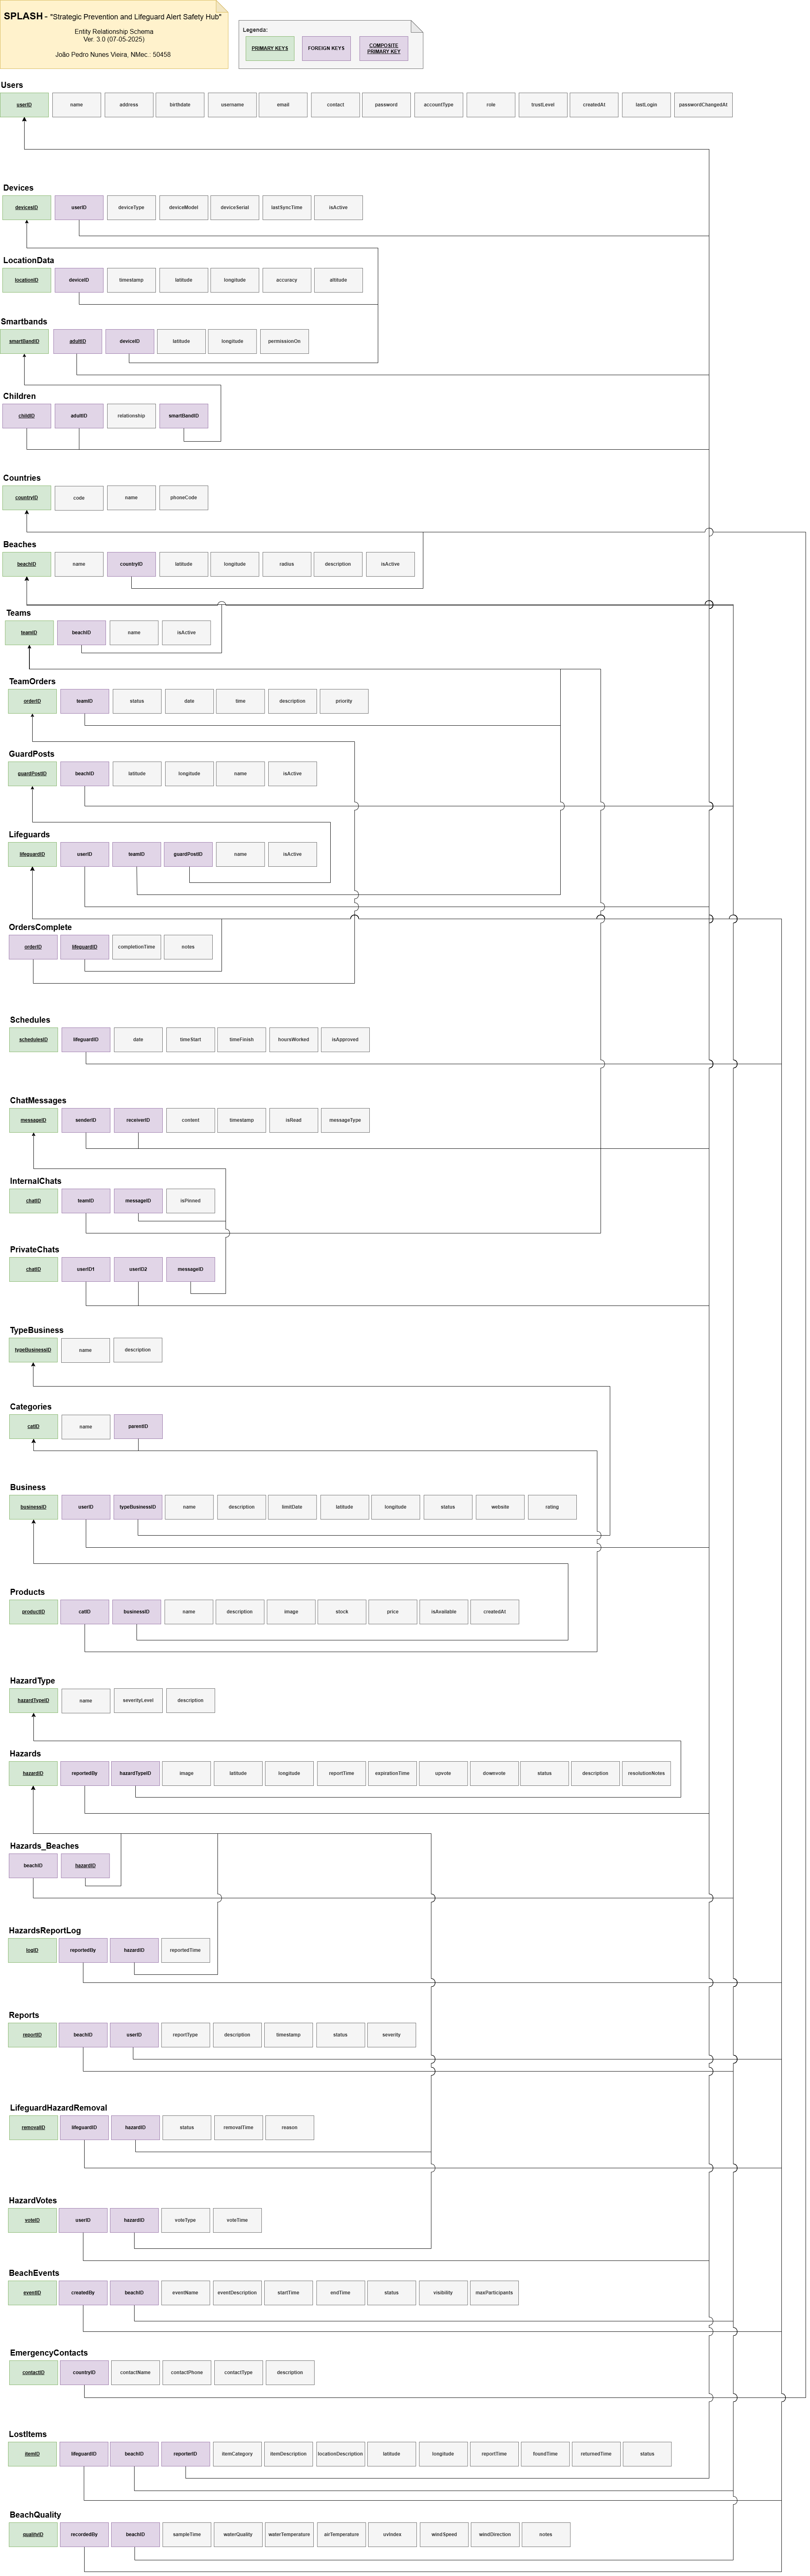
\includegraphics[width=6.5cm]{figs/Relational_Schema.png}
    \caption{\textbf{\ac{splash}: Relational Schema.} The schema translates the conceptual design into implementation-ready tables, complete with primary keys, foreign keys, and all necessary fields to support data integrity. For a more detailed view: \url{https://github.com/SPLASHub/SplashDocumentation/}}
    \label{fig:Relational_Schema}
\end{figure}

The relational schema provides a detailed logical blueprint for the implementation of the \ac{splash} database. Each table reflects a real-world entity and its attributes, and the schema incorporates comprehensive relationship mapping.

\textbf{Normalization and Integrity:}
\begin{itemize}
    \item Each table has a clearly defined primary key (e.g., \texttt{userID}, \texttt{hazardID}, \texttt{beachID}).
    \item Foreign keys enforce data consistency across related tables.
    \item Constraints such as \texttt{NOT NULL}, \texttt{UNIQUE}, and \texttt{CHECK} maintain the validity of data inputs.
    \item Attribute domains are defined with appropriate data types.
    \item No computed or derived fields are stored, in accordance with normalization principles.
\end{itemize}

\textbf{Performance and Optimization:}
\begin{itemize}
    \item Indexes are applied to fields used in joins and search conditions (e.g., foreign keys and commonly queried attributes).
    \item The schema allows for horizontal scaling (e.g. new rows) and vertical scaling (new columns or tables) without major structural revisions.
\end{itemize}

\textbf{Extensibility:} The modular and relational design enables future integrations with minimal disruption:
\begin{itemize}
    \item Additional smart devices can be added via the \texttt{Devices} or \texttt{Smartbands} tables.
    \item New user roles (e.g., medical responders, volunteers) can be appended by extending the \texttt{Users} entity and its relations.
    \item New environmental or safety data sources can be accommodated by expanding the \texttt{Hazards} or \texttt{LocationData} tables.
\end{itemize}

\subsection{SmartBand firmware}

The bracelet’s firmware implements a tightly choreographed startup sequence and task-based runtime architecture on the ESP32-S3-WROOM-1 using the \ac{ESPIDF} framework and \ac{FreeRTOS}. Upon power-up, the firmware first brings up the \ac{BLE} stack in peripheral role by initializing the NimBLE host and controller, configuring \ac{GAP} parameters—such as the device name “SPLASH\_BRACELET” and a 100 ms advertising interval—and registering a primary \ac{GATT} profile. The \ac{GATT} server then defines a Location and Speed service exposing two notifiable characteristics: a UTF-8 string carrying latitude and longitude in decimal degrees and a little-endian 32-bit integer representing speed in centimetres per second.

With \ac{BLE} advertising active, the application configures two \ac{UART} ports at 115 200 baud (\ac{UART}1 for the u-blox NEO-6M \ac{GPS} module and \ac{UART}2 for debug output) by installing interrupt-driven receive buffers and spawning the GPS\_UART\_Task. Immediately thereafter, the firmware programs the \ac{GPS} module for a 5 Hz update rate and optimized hot-start sensitivity by transmitting a sequence of \ac{UBX}-formatted configuration frames over \ac{UART}1. These commands enable only the \ac{GGA} and \ac{RMC} \ac{NMEA} sentences, reducing downstream parsing load.

\ac{FreeRTOS} then schedules the radio, host and \ac{GATT} subtasks alongside two application tasks. The GPS task blocks on incoming bytes from \ac{UART}1, aggregates complete \ac{NMEA} frames and hands them to the parser module, which validates checksums, fragments sentences and extracts fix data—latitude, longitude, UTC time, satellite count and speed. Parsed values write into a mutex-protected data structure, and each valid \ac{RMC} sentence triggers an event flag. The \ac{BLE} task waits on this event, then calls the \ac{GATT} update functions to write the new coordinate and speed values and issue notifications to any connected central device. Both tasks log errors via the ESP32 logging \ac{API} and, in the case of transient faults, retry after a brief non-blocking delay, ensuring the scheduler remains responsive.

By decoupling \ac{BLE} and \ac{GPS} workflows into independent, event-driven tasks, the firmware ensures that sensor polling, message parsing and radio event handling proceed concurrently without interference. The resulting data flow—from satellite signals to \ac{UART}, through \ac{NMEA} parsing into application state, and onward via \ac{GATT} notifications to a central client—runs at a steady five updates per second with sub-meter precision, all while drawing only milliamperes during active operation. This design satisfies the \ac{splash} ecosystem’s requirements for low-power, high-responsiveness child-tracking devices.
\subsection{Conclusion}
The \ac{splash} database design effectively balances real-world complexity with relational efficiency. Both the \ac{erd} and the implemented schema reflect strong adherence to database normalization principles, particularly up to Third Normal Form (3NF). The structure ensures minimal redundancy, optimized performance, and maintainability, while remaining adaptable.
    